\documentclass[twoside]{book}

% Packages required by doxygen
\usepackage{calc}
\usepackage{doxygen}
\usepackage{graphicx}
\usepackage[utf8]{inputenc}
\usepackage{makeidx}
\usepackage{multicol}
\usepackage{multirow}
\usepackage{textcomp}
\usepackage[table]{xcolor}

% Font selection
\usepackage[T1]{fontenc}
\usepackage{mathptmx}
\usepackage[scaled=.90]{helvet}
\usepackage{courier}
\usepackage{amssymb}
\usepackage{sectsty}
\renewcommand{\familydefault}{\sfdefault}
\allsectionsfont{%
  \fontseries{bc}\selectfont%
  \color{darkgray}%
}
\renewcommand{\DoxyLabelFont}{%
  \fontseries{bc}\selectfont%
  \color{darkgray}%
}

% Page & text layout
\usepackage{geometry}
\geometry{%
  a4paper,%
  top=2.5cm,%
  bottom=2.5cm,%
  left=2.5cm,%
  right=2.5cm%
}
\tolerance=750
\hfuzz=15pt
\hbadness=750
\setlength{\emergencystretch}{15pt}
\setlength{\parindent}{0cm}
\setlength{\parskip}{0.2cm}
\makeatletter
\renewcommand{\paragraph}{%
  \@startsection{paragraph}{4}{0ex}{-1.0ex}{1.0ex}{%
    \normalfont\normalsize\bfseries\SS@parafont%
  }%
}
\renewcommand{\subparagraph}{%
  \@startsection{subparagraph}{5}{0ex}{-1.0ex}{1.0ex}{%
    \normalfont\normalsize\bfseries\SS@subparafont%
  }%
}
\makeatother

% Headers & footers
\usepackage{fancyhdr}
\pagestyle{fancyplain}
\fancyhead[LE]{\fancyplain{}{\bfseries\thepage}}
\fancyhead[CE]{\fancyplain{}{}}
\fancyhead[RE]{\fancyplain{}{\bfseries\leftmark}}
\fancyhead[LO]{\fancyplain{}{\bfseries\rightmark}}
\fancyhead[CO]{\fancyplain{}{}}
\fancyhead[RO]{\fancyplain{}{\bfseries\thepage}}
\fancyfoot[LE]{\fancyplain{}{}}
\fancyfoot[CE]{\fancyplain{}{}}
\fancyfoot[RE]{\fancyplain{}{\bfseries\scriptsize Generated on Sun Jul 20 2014 23\-:43\-:02 for Sorting and Searching algorithms by Doxygen }}
\fancyfoot[LO]{\fancyplain{}{\bfseries\scriptsize Generated on Sun Jul 20 2014 23\-:43\-:02 for Sorting and Searching algorithms by Doxygen }}
\fancyfoot[CO]{\fancyplain{}{}}
\fancyfoot[RO]{\fancyplain{}{}}
\renewcommand{\footrulewidth}{0.4pt}
\renewcommand{\chaptermark}[1]{%
  \markboth{#1}{}%
}
\renewcommand{\sectionmark}[1]{%
  \markright{\thesection\ #1}%
}

% Indices & bibliography
\usepackage{natbib}
\usepackage[titles]{tocloft}
\setcounter{tocdepth}{3}
\setcounter{secnumdepth}{5}
\makeindex

% Hyperlinks (required, but should be loaded last)
\usepackage{ifpdf}
\ifpdf
  \usepackage[pdftex,pagebackref=true]{hyperref}
\else
  \usepackage[ps2pdf,pagebackref=true]{hyperref}
\fi
\hypersetup{%
  colorlinks=true,%
  linkcolor=blue,%
  citecolor=blue,%
  unicode%
}

% Custom commands
\newcommand{\clearemptydoublepage}{%
  \newpage{\pagestyle{empty}\cleardoublepage}%
}


%===== C O N T E N T S =====

\begin{document}

% Titlepage & ToC
\hypersetup{pageanchor=false}
\pagenumbering{roman}
\begin{titlepage}
\vspace*{7cm}
\begin{center}%
{\Large Sorting and Searching algorithms }\\
\vspace*{1cm}
{\large Generated by Doxygen 1.8.6}\\
\vspace*{0.5cm}
{\small Sun Jul 20 2014 23:43:02}\\
\end{center}
\end{titlepage}
\clearemptydoublepage
\tableofcontents
\clearemptydoublepage
\pagenumbering{arabic}
\hypersetup{pageanchor=true}

%--- Begin generated contents ---
\chapter{Main page}
\label{index}\hypertarget{index}{}\hypertarget{index_intro_sec}{}\section{Purpose}\label{index_intro_sec}
This is a project for the course Data Structures at the Computer Engineering and Informatics Department, University of Patras. The purpose of this project was to implement basic sorting and searching algorithms.\hypertarget{index_compile_sec}{}\section{Compiling}\label{index_compile_sec}
\begin{center} mkdir build \&\& cd build \&\& cmake .. \&\& make \&\& cd .. \end{center} \hypertarget{index_run_sec}{}\section{Running}\label{index_run_sec}
\begin{center} cd bin \&\& ./sort\-Nsearch \end{center} \hypertarget{index_dep_sec}{}\section{Dependancies (\-Debian based systems)}\label{index_dep_sec}
\begin{center} sudo apt-\/get install cmake (Minimum version 2.\-6 required) \end{center} \hypertarget{index_info_sec}{}\section{More information}\label{index_info_sec}
Contact\-: \href{mailto:b.papaspyros@gmail.com}{\tt b.\-papaspyros@gmail.\-com} or create an issue on the github page \href{https://github.com/bpapaspyros/DataStructures}{\tt https\-://github.\-com/bpapaspyros/\-Data\-Structures}

\begin{DoxyAuthor}{Author}
Vaios Papaspyros 
\end{DoxyAuthor}

\chapter{Class Index}
\section{Class List}
Here are the classes, structs, unions and interfaces with brief descriptions\-:\begin{DoxyCompactList}
\item\contentsline{section}{\hyperlink{class_graph_vis}{Graph\-Vis} \\*\hyperlink{class_graph_vis}{Graph\-Vis} Class }{\pageref{class_graph_vis}}{}
\item\contentsline{section}{\hyperlink{class_interface}{Interface} \\*\hyperlink{class_interface}{Interface} Class }{\pageref{class_interface}}{}
\item\contentsline{section}{\hyperlink{class_node}{Node} \\*\hyperlink{class_node}{Node} Class }{\pageref{class_node}}{}
\item\contentsline{section}{\hyperlink{class_tree}{Tree} \\*\hyperlink{class_tree}{Tree} Class }{\pageref{class_tree}}{}
\end{DoxyCompactList}

\chapter{File Index}
\section{File List}
Here is a list of all files with brief descriptions\-:\begin{DoxyCompactList}
\item\contentsline{section}{/home/baios/\-Coding/\-C++/\-Git\-Data\-Structures/\-Data\-Structures/234\-Tree/build/\-C\-Make\-Files/2.\-8.\-12.\-2/\-Compiler\-Id\-C/\hyperlink{_c_make_c_compiler_id_8c}{C\-Make\-C\-Compiler\-Id.\-c} }{\pageref{_c_make_c_compiler_id_8c}}{}
\item\contentsline{section}{/home/baios/\-Coding/\-C++/\-Git\-Data\-Structures/\-Data\-Structures/234\-Tree/build/\-C\-Make\-Files/2.\-8.\-12.\-2/\-Compiler\-Id\-C\-X\-X/\hyperlink{_c_make_c_x_x_compiler_id_8cpp}{C\-Make\-C\-X\-X\-Compiler\-Id.\-cpp} }{\pageref{_c_make_c_x_x_compiler_id_8cpp}}{}
\item\contentsline{section}{/home/baios/\-Coding/\-C++/\-Git\-Data\-Structures/\-Data\-Structures/234\-Tree/include/\hyperlink{_graph_vis_8h}{Graph\-Vis.\-h} }{\pageref{_graph_vis_8h}}{}
\item\contentsline{section}{/home/baios/\-Coding/\-C++/\-Git\-Data\-Structures/\-Data\-Structures/234\-Tree/include/\hyperlink{_interface_8h}{Interface.\-h} }{\pageref{_interface_8h}}{}
\item\contentsline{section}{/home/baios/\-Coding/\-C++/\-Git\-Data\-Structures/\-Data\-Structures/234\-Tree/include/\hyperlink{_node_8h}{Node.\-h} }{\pageref{_node_8h}}{}
\item\contentsline{section}{/home/baios/\-Coding/\-C++/\-Git\-Data\-Structures/\-Data\-Structures/234\-Tree/include/\hyperlink{_tree_8h}{Tree.\-h} }{\pageref{_tree_8h}}{}
\item\contentsline{section}{/home/baios/\-Coding/\-C++/\-Git\-Data\-Structures/\-Data\-Structures/234\-Tree/src/\hyperlink{_graph_vis_8cpp}{Graph\-Vis.\-cpp} }{\pageref{_graph_vis_8cpp}}{}
\item\contentsline{section}{/home/baios/\-Coding/\-C++/\-Git\-Data\-Structures/\-Data\-Structures/234\-Tree/src/\hyperlink{_interface_8cpp}{Interface.\-cpp} }{\pageref{_interface_8cpp}}{}
\item\contentsline{section}{/home/baios/\-Coding/\-C++/\-Git\-Data\-Structures/\-Data\-Structures/234\-Tree/src/\hyperlink{main_8cpp}{main.\-cpp} }{\pageref{main_8cpp}}{}
\item\contentsline{section}{/home/baios/\-Coding/\-C++/\-Git\-Data\-Structures/\-Data\-Structures/234\-Tree/src/\hyperlink{_node_8cpp}{Node.\-cpp} }{\pageref{_node_8cpp}}{}
\item\contentsline{section}{/home/baios/\-Coding/\-C++/\-Git\-Data\-Structures/\-Data\-Structures/234\-Tree/src/\hyperlink{_tree_8cpp}{Tree.\-cpp} }{\pageref{_tree_8cpp}}{}
\end{DoxyCompactList}

\chapter{Class Documentation}
\hypertarget{class_sort___n___search}{\section{Sort\-\_\-\-N\-\_\-\-Search Class Reference}
\label{class_sort___n___search}\index{Sort\-\_\-\-N\-\_\-\-Search@{Sort\-\_\-\-N\-\_\-\-Search}}
}


Sorting and Searching algorithms.  




{\ttfamily \#include $<$Sort\-\_\-\-N\-\_\-\-Search.\-h$>$}

\subsection*{Public Member Functions}
\begin{DoxyCompactItemize}
\item 
\hyperlink{class_sort___n___search_acf81cd769d970ce94376d7303bc5b7c9}{Sort\-\_\-\-N\-\_\-\-Search} ()
\begin{DoxyCompactList}\small\item\em Constructor. \end{DoxyCompactList}\item 
void \hyperlink{class_sort___n___search_ad34f3e05b8ed39ea004e7253b7d7c068}{mergesort} (int $\ast$in\-Array, int lower\-\_\-lim, int upper\-\_\-lim)
\begin{DoxyCompactList}\small\item\em M\-E\-R\-G\-E\-S\-O\-R\-T implementation. The basic idea behind the mergesort algorithm is that we split the initial array that we are given in to two equal arrays recursively until we come to have two numbers and then we sort those and merge them into a single array (the original one that we were given) \end{DoxyCompactList}\item 
void \hyperlink{class_sort___n___search_a92480efea81ee755f6353d9a2e96ee03}{merge} (int $\ast$in\-Array, int lower\-\_\-lim, int upper\-\_\-lim)
\begin{DoxyCompactList}\small\item\em Merge. \end{DoxyCompactList}\item 
void \hyperlink{class_sort___n___search_a6bfaafde8113af23379d2e2091531c5a}{quicksort} (int $\ast$in\-Array, int lower\-\_\-lim, int upper\-\_\-lim)
\begin{DoxyCompactList}\small\item\em Q\-U\-I\-C\-K\-S\-O\-R\-T implementation. \end{DoxyCompactList}\item 
void \hyperlink{class_sort___n___search_a3673aa59d2adfdec3e4b6ea2392b8398}{bublesort} (int $\ast$in\-Array, int size)
\begin{DoxyCompactList}\small\item\em B\-U\-B\-L\-E\-S\-O\-R\-T implementation. \end{DoxyCompactList}\item 
int \hyperlink{class_sort___n___search_ac5b19bdbc68b7a4eeb4b0fd5d3256190}{binary\-Search} (int $\ast$in\-Array, int lower\-\_\-limit, int upper\-\_\-limit, int key)
\begin{DoxyCompactList}\small\item\em B\-I\-N\-A\-R\-Y implementation. \end{DoxyCompactList}\item 
int \hyperlink{class_sort___n___search_a6597cc2fc0e04fa9ccc0855dc2e07d1c}{binary\-Interpolation\-Search} (int $\ast$in\-Array, int size, int key)
\begin{DoxyCompactList}\small\item\em B\-I\-N\-A\-R\-Y I\-N\-T\-E\-R\-P\-O\-L\-A\-T\-I\-O\-N implementation. \end{DoxyCompactList}\item 
void \hyperlink{class_sort___n___search_a63c1e873a63857191d90c088147ee083}{print\-Menu} (int el\-Num)
\begin{DoxyCompactList}\small\item\em A C\-L\-I built so that the user can choose between sorting and searching algorithms, as well as input filenames and search keys. \end{DoxyCompactList}\item 
void \hyperlink{class_sort___n___search_a7cf521f21bdcb5febabf4b0f6a032e1d}{print\-Array} (int $\ast$in\-Array, int size)
\begin{DoxyCompactList}\small\item\em Prints the array give to the console. \end{DoxyCompactList}\item 
double \hyperlink{class_sort___n___search_a842553953c3f0d3b6a787b7669e0a26e}{get\-Execution\-Time} ()
\begin{DoxyCompactList}\small\item\em Returns the execution time. \end{DoxyCompactList}\end{DoxyCompactItemize}


\subsection{Detailed Description}
Sorting and Searching algorithms. 

This class contains three sorting algorithms (Mergesort, Quicksort, Bublesort) and two searching (Binary and Binary Interpolation). The above algotithms are designed to be used with integers. There have also been implemented methods for reading and writing data from/to files, methods that allow the programmer to meassure the execution time of any of the above algorithms. There are also methods that intialize an array with random integers as well as a basic C\-L\-I for the user.

\begin{DoxyAuthor}{Author}
Vaios Papaspyros
\end{DoxyAuthor}
Contact\-: \href{mailto:b.papaspyros@gmail.com}{\tt b.\-papaspyros@gmail.\-com} or create an issue on the github page \href{https://github.com/bpapaspyros/DataStructures}{\tt https\-://github.\-com/bpapaspyros/\-Data\-Structures} 

Definition at line 31 of file Sort\-\_\-\-N\-\_\-\-Search.\-h.



\subsection{Constructor \& Destructor Documentation}
\hypertarget{class_sort___n___search_acf81cd769d970ce94376d7303bc5b7c9}{\index{Sort\-\_\-\-N\-\_\-\-Search@{Sort\-\_\-\-N\-\_\-\-Search}!Sort\-\_\-\-N\-\_\-\-Search@{Sort\-\_\-\-N\-\_\-\-Search}}
\index{Sort\-\_\-\-N\-\_\-\-Search@{Sort\-\_\-\-N\-\_\-\-Search}!Sort_N_Search@{Sort\-\_\-\-N\-\_\-\-Search}}
\subsubsection[{Sort\-\_\-\-N\-\_\-\-Search}]{\setlength{\rightskip}{0pt plus 5cm}Sort\-\_\-\-N\-\_\-\-Search\-::\-Sort\-\_\-\-N\-\_\-\-Search (
\begin{DoxyParamCaption}
{}
\end{DoxyParamCaption}
)}}\label{class_sort___n___search_acf81cd769d970ce94376d7303bc5b7c9}


Constructor. 

Initalizing time values to the defaults 

Definition at line 4 of file Sort\-\_\-\-N\-\_\-\-Search.\-cpp.



\subsection{Member Function Documentation}
\hypertarget{class_sort___n___search_a6597cc2fc0e04fa9ccc0855dc2e07d1c}{\index{Sort\-\_\-\-N\-\_\-\-Search@{Sort\-\_\-\-N\-\_\-\-Search}!binary\-Interpolation\-Search@{binary\-Interpolation\-Search}}
\index{binary\-Interpolation\-Search@{binary\-Interpolation\-Search}!Sort_N_Search@{Sort\-\_\-\-N\-\_\-\-Search}}
\subsubsection[{binary\-Interpolation\-Search}]{\setlength{\rightskip}{0pt plus 5cm}int Sort\-\_\-\-N\-\_\-\-Search\-::binary\-Interpolation\-Search (
\begin{DoxyParamCaption}
\item[{int $\ast$}]{in\-Array, }
\item[{int}]{size, }
\item[{int}]{key}
\end{DoxyParamCaption}
)}}\label{class_sort___n___search_a6597cc2fc0e04fa9ccc0855dc2e07d1c}


B\-I\-N\-A\-R\-Y I\-N\-T\-E\-R\-P\-O\-L\-A\-T\-I\-O\-N implementation. 


\begin{DoxyParams}{Parameters}
{\em An} & array with our elements, its size and the search key given by the user\\
\hline
\end{DoxyParams}
\begin{DoxyReturn}{Returns}
The index where the key was found or a -\/1 indicating the key was not found
\end{DoxyReturn}
The basic idea behind the binary interpolation search algorithm is that we combine the benefits of applying a binary and an interpolation search so that we narrow down the search key in less loops. There has been added a code snippet to check if the initial next variable is out of bounds for our array 

Definition at line 185 of file Sort\-\_\-\-N\-\_\-\-Search.\-cpp.



Here is the caller graph for this function\-:\nopagebreak
\begin{figure}[H]
\begin{center}
\leavevmode
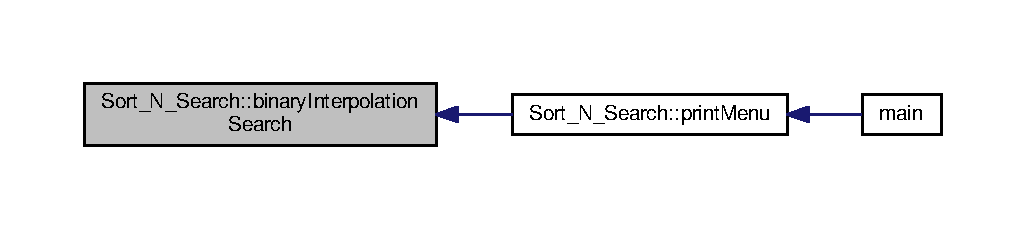
\includegraphics[width=350pt]{class_sort___n___search_a6597cc2fc0e04fa9ccc0855dc2e07d1c_icgraph}
\end{center}
\end{figure}


\hypertarget{class_sort___n___search_ac5b19bdbc68b7a4eeb4b0fd5d3256190}{\index{Sort\-\_\-\-N\-\_\-\-Search@{Sort\-\_\-\-N\-\_\-\-Search}!binary\-Search@{binary\-Search}}
\index{binary\-Search@{binary\-Search}!Sort_N_Search@{Sort\-\_\-\-N\-\_\-\-Search}}
\subsubsection[{binary\-Search}]{\setlength{\rightskip}{0pt plus 5cm}int Sort\-\_\-\-N\-\_\-\-Search\-::binary\-Search (
\begin{DoxyParamCaption}
\item[{int $\ast$}]{in\-Array, }
\item[{int}]{lower\-\_\-limit, }
\item[{int}]{upper\-\_\-limit, }
\item[{int}]{key}
\end{DoxyParamCaption}
)}}\label{class_sort___n___search_ac5b19bdbc68b7a4eeb4b0fd5d3256190}


B\-I\-N\-A\-R\-Y implementation. 


\begin{DoxyParams}{Parameters}
{\em An} & array with our elements, two integers representing the upper and lower limit of the array and the search key given by the user\\
\hline
\end{DoxyParams}
\begin{DoxyReturn}{Returns}
The index where the key was found or a -\/1 indicating the key was not found
\end{DoxyReturn}
The basic idea behind the binary search algorithm is that we check the middle value of the array and if it is smaller than the key given then we search recursively the right half of the array otherwise we search the right part, unless the key give is located in the middle 

Definition at line 155 of file Sort\-\_\-\-N\-\_\-\-Search.\-cpp.



Here is the caller graph for this function\-:\nopagebreak
\begin{figure}[H]
\begin{center}
\leavevmode
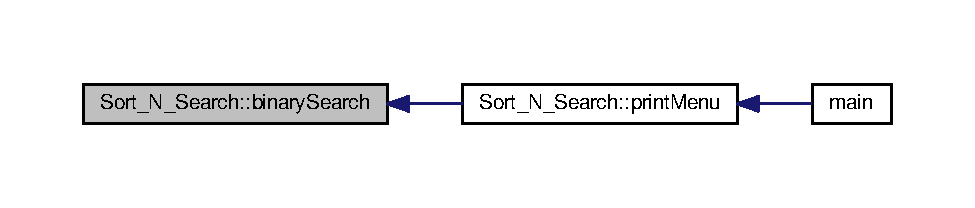
\includegraphics[width=350pt]{class_sort___n___search_ac5b19bdbc68b7a4eeb4b0fd5d3256190_icgraph}
\end{center}
\end{figure}


\hypertarget{class_sort___n___search_a3673aa59d2adfdec3e4b6ea2392b8398}{\index{Sort\-\_\-\-N\-\_\-\-Search@{Sort\-\_\-\-N\-\_\-\-Search}!bublesort@{bublesort}}
\index{bublesort@{bublesort}!Sort_N_Search@{Sort\-\_\-\-N\-\_\-\-Search}}
\subsubsection[{bublesort}]{\setlength{\rightskip}{0pt plus 5cm}void Sort\-\_\-\-N\-\_\-\-Search\-::bublesort (
\begin{DoxyParamCaption}
\item[{int $\ast$}]{in\-Array, }
\item[{int}]{size}
\end{DoxyParamCaption}
)}}\label{class_sort___n___search_a3673aa59d2adfdec3e4b6ea2392b8398}


B\-U\-B\-L\-E\-S\-O\-R\-T implementation. 


\begin{DoxyParams}{Parameters}
{\em An} & array with our elements and its size\\
\hline
\end{DoxyParams}
The basic idea behind the bublesort algorithm is that we scan the whole array until we find the min value and then we use the same method with the next min value until all elements are sorted 

Definition at line 121 of file Sort\-\_\-\-N\-\_\-\-Search.\-cpp.



Here is the caller graph for this function\-:\nopagebreak
\begin{figure}[H]
\begin{center}
\leavevmode
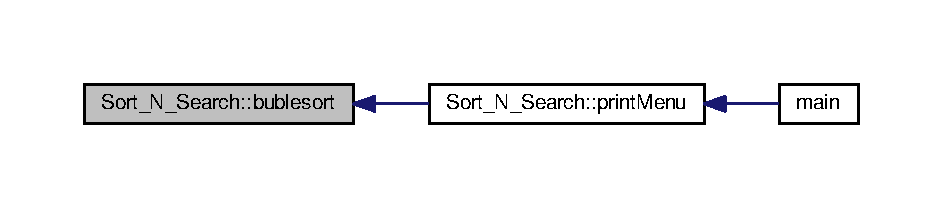
\includegraphics[width=350pt]{class_sort___n___search_a3673aa59d2adfdec3e4b6ea2392b8398_icgraph}
\end{center}
\end{figure}


\hypertarget{class_sort___n___search_a842553953c3f0d3b6a787b7669e0a26e}{\index{Sort\-\_\-\-N\-\_\-\-Search@{Sort\-\_\-\-N\-\_\-\-Search}!get\-Execution\-Time@{get\-Execution\-Time}}
\index{get\-Execution\-Time@{get\-Execution\-Time}!Sort_N_Search@{Sort\-\_\-\-N\-\_\-\-Search}}
\subsubsection[{get\-Execution\-Time}]{\setlength{\rightskip}{0pt plus 5cm}double Sort\-\_\-\-N\-\_\-\-Search\-::get\-Execution\-Time (
\begin{DoxyParamCaption}
{}
\end{DoxyParamCaption}
)}}\label{class_sort___n___search_a842553953c3f0d3b6a787b7669e0a26e}


Returns the execution time. 

\begin{DoxyReturn}{Returns}
Execution time meassured 
\end{DoxyReturn}


Definition at line 377 of file Sort\-\_\-\-N\-\_\-\-Search.\-cpp.

\hypertarget{class_sort___n___search_a92480efea81ee755f6353d9a2e96ee03}{\index{Sort\-\_\-\-N\-\_\-\-Search@{Sort\-\_\-\-N\-\_\-\-Search}!merge@{merge}}
\index{merge@{merge}!Sort_N_Search@{Sort\-\_\-\-N\-\_\-\-Search}}
\subsubsection[{merge}]{\setlength{\rightskip}{0pt plus 5cm}void Sort\-\_\-\-N\-\_\-\-Search\-::merge (
\begin{DoxyParamCaption}
\item[{int $\ast$}]{in\-Array, }
\item[{int}]{lower\-\_\-lim, }
\item[{int}]{upper\-\_\-lim}
\end{DoxyParamCaption}
)}}\label{class_sort___n___search_a92480efea81ee755f6353d9a2e96ee03}


Merge. 

Merges two sub arrays into one that is sorted


\begin{DoxyParams}{Parameters}
{\em An} & array with our elements and two integers representing the upper and lower limit of the array \\
\hline
\end{DoxyParams}


Definition at line 33 of file Sort\-\_\-\-N\-\_\-\-Search.\-cpp.



Here is the caller graph for this function\-:\nopagebreak
\begin{figure}[H]
\begin{center}
\leavevmode
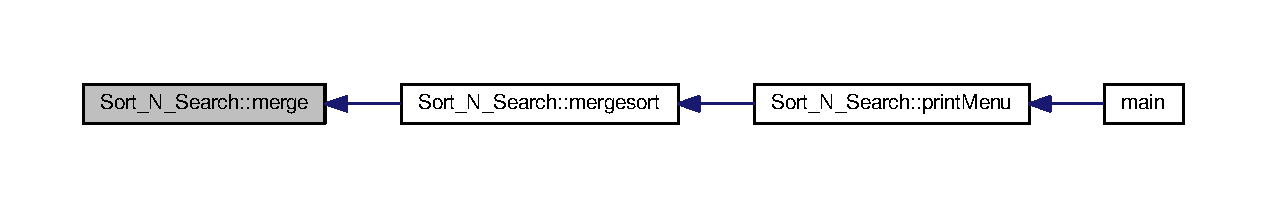
\includegraphics[width=350pt]{class_sort___n___search_a92480efea81ee755f6353d9a2e96ee03_icgraph}
\end{center}
\end{figure}


\hypertarget{class_sort___n___search_ad34f3e05b8ed39ea004e7253b7d7c068}{\index{Sort\-\_\-\-N\-\_\-\-Search@{Sort\-\_\-\-N\-\_\-\-Search}!mergesort@{mergesort}}
\index{mergesort@{mergesort}!Sort_N_Search@{Sort\-\_\-\-N\-\_\-\-Search}}
\subsubsection[{mergesort}]{\setlength{\rightskip}{0pt plus 5cm}void Sort\-\_\-\-N\-\_\-\-Search\-::mergesort (
\begin{DoxyParamCaption}
\item[{int $\ast$}]{in\-Array, }
\item[{int}]{lower\-\_\-lim, }
\item[{int}]{upper\-\_\-lim}
\end{DoxyParamCaption}
)}}\label{class_sort___n___search_ad34f3e05b8ed39ea004e7253b7d7c068}


M\-E\-R\-G\-E\-S\-O\-R\-T implementation. The basic idea behind the mergesort algorithm is that we split the initial array that we are given in to two equal arrays recursively until we come to have two numbers and then we sort those and merge them into a single array (the original one that we were given) 


\begin{DoxyParams}{Parameters}
{\em An} & array with our elements and two integers representing the upper and lower limit of the array \\
\hline
\end{DoxyParams}


Definition at line 25 of file Sort\-\_\-\-N\-\_\-\-Search.\-cpp.



Here is the call graph for this function\-:\nopagebreak
\begin{figure}[H]
\begin{center}
\leavevmode
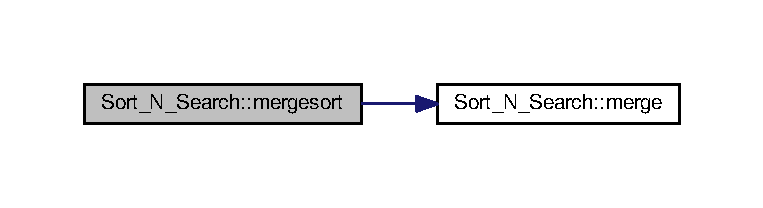
\includegraphics[width=350pt]{class_sort___n___search_ad34f3e05b8ed39ea004e7253b7d7c068_cgraph}
\end{center}
\end{figure}




Here is the caller graph for this function\-:\nopagebreak
\begin{figure}[H]
\begin{center}
\leavevmode
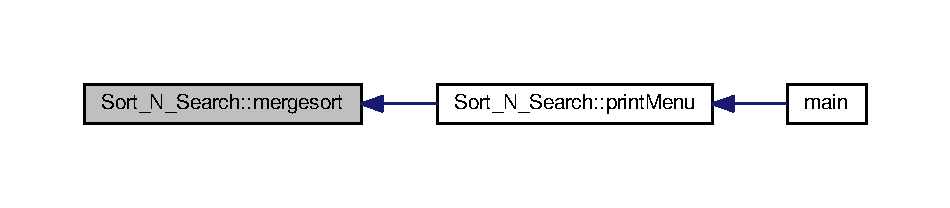
\includegraphics[width=350pt]{class_sort___n___search_ad34f3e05b8ed39ea004e7253b7d7c068_icgraph}
\end{center}
\end{figure}


\hypertarget{class_sort___n___search_a7cf521f21bdcb5febabf4b0f6a032e1d}{\index{Sort\-\_\-\-N\-\_\-\-Search@{Sort\-\_\-\-N\-\_\-\-Search}!print\-Array@{print\-Array}}
\index{print\-Array@{print\-Array}!Sort_N_Search@{Sort\-\_\-\-N\-\_\-\-Search}}
\subsubsection[{print\-Array}]{\setlength{\rightskip}{0pt plus 5cm}void Sort\-\_\-\-N\-\_\-\-Search\-::print\-Array (
\begin{DoxyParamCaption}
\item[{int $\ast$}]{in\-Array, }
\item[{int}]{size}
\end{DoxyParamCaption}
)}}\label{class_sort___n___search_a7cf521f21bdcb5febabf4b0f6a032e1d}


Prints the array give to the console. 


\begin{DoxyParams}{Parameters}
{\em An} & array and its size \\
\hline
\end{DoxyParams}


Definition at line 391 of file Sort\-\_\-\-N\-\_\-\-Search.\-cpp.

\hypertarget{class_sort___n___search_a63c1e873a63857191d90c088147ee083}{\index{Sort\-\_\-\-N\-\_\-\-Search@{Sort\-\_\-\-N\-\_\-\-Search}!print\-Menu@{print\-Menu}}
\index{print\-Menu@{print\-Menu}!Sort_N_Search@{Sort\-\_\-\-N\-\_\-\-Search}}
\subsubsection[{print\-Menu}]{\setlength{\rightskip}{0pt plus 5cm}void Sort\-\_\-\-N\-\_\-\-Search\-::print\-Menu (
\begin{DoxyParamCaption}
\item[{int}]{el\-Num}
\end{DoxyParamCaption}
)}}\label{class_sort___n___search_a63c1e873a63857191d90c088147ee083}


A C\-L\-I built so that the user can choose between sorting and searching algorithms, as well as input filenames and search keys. 


\begin{DoxyParams}{Parameters}
{\em Number} & of elements in the array passed from the main fucntion \\
\hline
\end{DoxyParams}


Definition at line 421 of file Sort\-\_\-\-N\-\_\-\-Search.\-cpp.



Here is the call graph for this function\-:\nopagebreak
\begin{figure}[H]
\begin{center}
\leavevmode
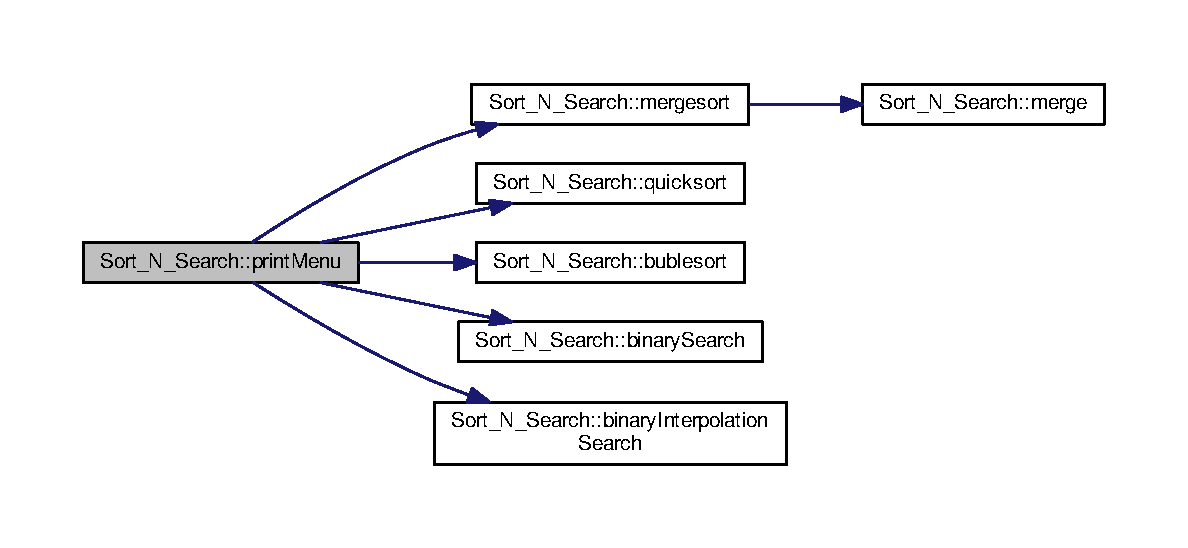
\includegraphics[width=350pt]{class_sort___n___search_a63c1e873a63857191d90c088147ee083_cgraph}
\end{center}
\end{figure}




Here is the caller graph for this function\-:\nopagebreak
\begin{figure}[H]
\begin{center}
\leavevmode
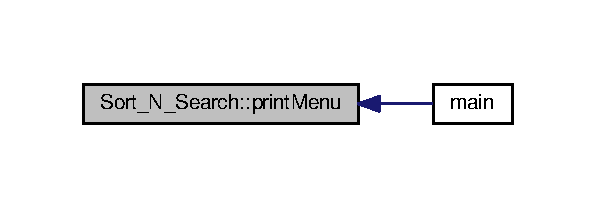
\includegraphics[width=286pt]{class_sort___n___search_a63c1e873a63857191d90c088147ee083_icgraph}
\end{center}
\end{figure}


\hypertarget{class_sort___n___search_a6bfaafde8113af23379d2e2091531c5a}{\index{Sort\-\_\-\-N\-\_\-\-Search@{Sort\-\_\-\-N\-\_\-\-Search}!quicksort@{quicksort}}
\index{quicksort@{quicksort}!Sort_N_Search@{Sort\-\_\-\-N\-\_\-\-Search}}
\subsubsection[{quicksort}]{\setlength{\rightskip}{0pt plus 5cm}void Sort\-\_\-\-N\-\_\-\-Search\-::quicksort (
\begin{DoxyParamCaption}
\item[{int $\ast$}]{in\-Array, }
\item[{int}]{lower\-\_\-lim, }
\item[{int}]{upper\-\_\-lim}
\end{DoxyParamCaption}
)}}\label{class_sort___n___search_a6bfaafde8113af23379d2e2091531c5a}


Q\-U\-I\-C\-K\-S\-O\-R\-T implementation. 


\begin{DoxyParams}{Parameters}
{\em An} & array with our elements and two integers representing the upper and lower limit of the array\\
\hline
\end{DoxyParams}
The basic idea behind the quicksort algorithm is that we use the divide and conquer method. We initially split the array to two arrays and then we apply the same method to the sub arrays recursively until the we get all elements sorted. 

Definition at line 78 of file Sort\-\_\-\-N\-\_\-\-Search.\-cpp.



Here is the caller graph for this function\-:\nopagebreak
\begin{figure}[H]
\begin{center}
\leavevmode
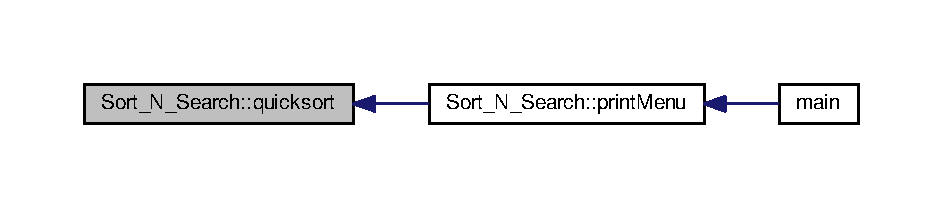
\includegraphics[width=350pt]{class_sort___n___search_a6bfaafde8113af23379d2e2091531c5a_icgraph}
\end{center}
\end{figure}




The documentation for this class was generated from the following files\-:\begin{DoxyCompactItemize}
\item 
/home/baios/\-Desktop/\-Git\-Data\-Structures/\-Data\-Structures/\-Sorting\-And\-Searching/include/\hyperlink{_sort___n___search_8h}{Sort\-\_\-\-N\-\_\-\-Search.\-h}\item 
/home/baios/\-Desktop/\-Git\-Data\-Structures/\-Data\-Structures/\-Sorting\-And\-Searching/src/\hyperlink{_sort___n___search_8cpp}{Sort\-\_\-\-N\-\_\-\-Search.\-cpp}\end{DoxyCompactItemize}

\chapter{File Documentation}
\hypertarget{_sort___n___search_8h}{\section{/home/baios/\-Desktop/\-Git\-Data\-Structures/\-Data\-Structures/\-Sorting\-And\-Searching/include/\-Sort\-\_\-\-N\-\_\-\-Search.h File Reference}
\label{_sort___n___search_8h}\index{/home/baios/\-Desktop/\-Git\-Data\-Structures/\-Data\-Structures/\-Sorting\-And\-Searching/include/\-Sort\-\_\-\-N\-\_\-\-Search.\-h@{/home/baios/\-Desktop/\-Git\-Data\-Structures/\-Data\-Structures/\-Sorting\-And\-Searching/include/\-Sort\-\_\-\-N\-\_\-\-Search.\-h}}
}
{\ttfamily \#include $<$iostream$>$}\\*
{\ttfamily \#include $<$cmath$>$}\\*
{\ttfamily \#include $<$ctime$>$}\\*
{\ttfamily \#include $<$cstdlib$>$}\\*
{\ttfamily \#include $<$fstream$>$}\\*
{\ttfamily \#include $<$cstring$>$}\\*
Include dependency graph for Sort\-\_\-\-N\-\_\-\-Search.\-h\-:\nopagebreak
\begin{figure}[H]
\begin{center}
\leavevmode
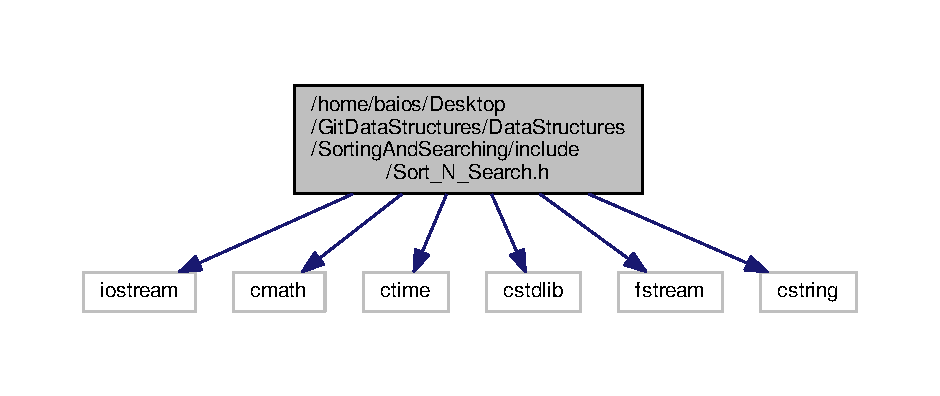
\includegraphics[width=350pt]{_sort___n___search_8h__incl}
\end{center}
\end{figure}
This graph shows which files directly or indirectly include this file\-:\nopagebreak
\begin{figure}[H]
\begin{center}
\leavevmode
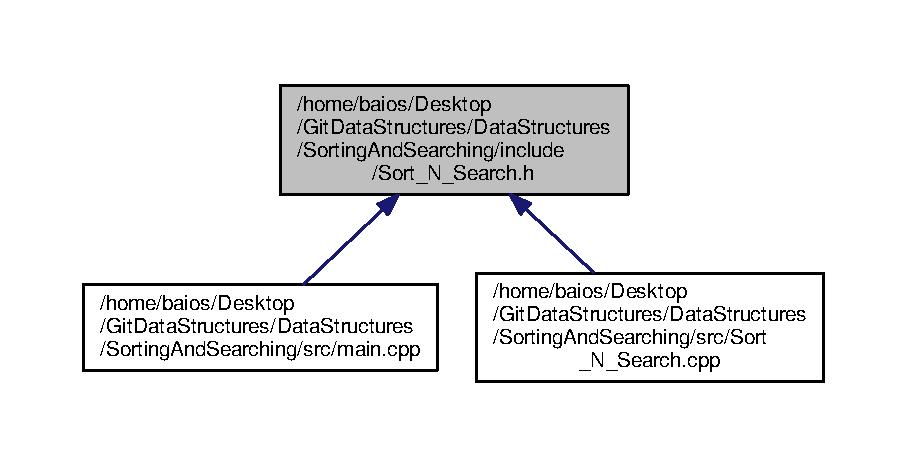
\includegraphics[width=350pt]{_sort___n___search_8h__dep__incl}
\end{center}
\end{figure}
\subsection*{Classes}
\begin{DoxyCompactItemize}
\item 
class \hyperlink{class_sort___n___search}{Sort\-\_\-\-N\-\_\-\-Search}
\begin{DoxyCompactList}\small\item\em Sorting and Searching algorithms. \end{DoxyCompactList}\end{DoxyCompactItemize}

\hypertarget{main_8cpp}{\section{/home/baios/\-Desktop/\-Git\-Data\-Structures/\-Data\-Structures/\-Sorting\-And\-Searching/src/main.cpp File Reference}
\label{main_8cpp}\index{/home/baios/\-Desktop/\-Git\-Data\-Structures/\-Data\-Structures/\-Sorting\-And\-Searching/src/main.\-cpp@{/home/baios/\-Desktop/\-Git\-Data\-Structures/\-Data\-Structures/\-Sorting\-And\-Searching/src/main.\-cpp}}
}
{\ttfamily \#include \char`\"{}Sort\-\_\-\-N\-\_\-\-Search.\-h\char`\"{}}\\*
Include dependency graph for main.\-cpp\-:\nopagebreak
\begin{figure}[H]
\begin{center}
\leavevmode
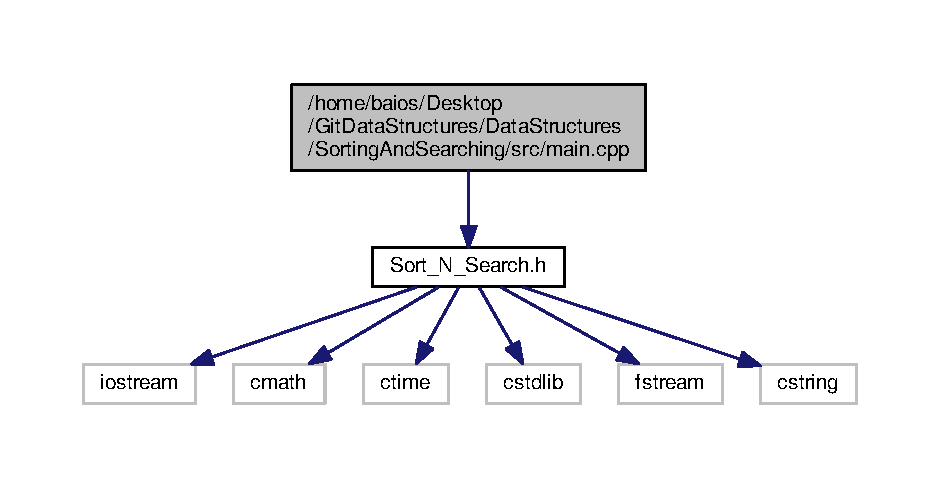
\includegraphics[width=350pt]{main_8cpp__incl}
\end{center}
\end{figure}
\subsection*{Functions}
\begin{DoxyCompactItemize}
\item 
int \hyperlink{main_8cpp_a3c04138a5bfe5d72780bb7e82a18e627}{main} (int argc, char $\ast$$\ast$argv)
\end{DoxyCompactItemize}


\subsection{Function Documentation}
\hypertarget{main_8cpp_a3c04138a5bfe5d72780bb7e82a18e627}{\index{main.\-cpp@{main.\-cpp}!main@{main}}
\index{main@{main}!main.cpp@{main.\-cpp}}
\subsubsection[{main}]{\setlength{\rightskip}{0pt plus 5cm}int main (
\begin{DoxyParamCaption}
\item[{int}]{argc, }
\item[{char $\ast$$\ast$}]{argv}
\end{DoxyParamCaption}
)}}\label{main_8cpp_a3c04138a5bfe5d72780bb7e82a18e627}

\begin{DoxyParams}{Parameters}
{\em Takes} & in an integer which represents the array size. \\
\hline
\end{DoxyParams}


Definition at line 33 of file main.\-cpp.



Here is the call graph for this function\-:\nopagebreak
\begin{figure}[H]
\begin{center}
\leavevmode
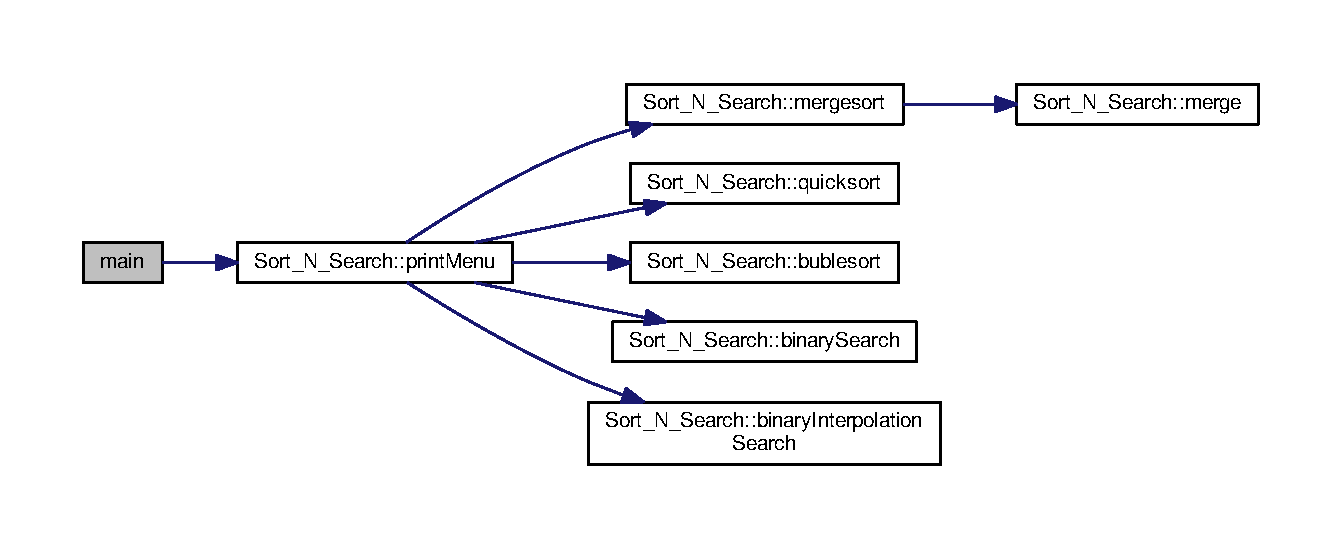
\includegraphics[width=350pt]{main_8cpp_a3c04138a5bfe5d72780bb7e82a18e627_cgraph}
\end{center}
\end{figure}



\hypertarget{_sort___n___search_8cpp}{\section{/home/baios/\-Desktop/\-Git\-Data\-Structures/\-Data\-Structures/\-Sorting\-And\-Searching/src/\-Sort\-\_\-\-N\-\_\-\-Search.cpp File Reference}
\label{_sort___n___search_8cpp}\index{/home/baios/\-Desktop/\-Git\-Data\-Structures/\-Data\-Structures/\-Sorting\-And\-Searching/src/\-Sort\-\_\-\-N\-\_\-\-Search.\-cpp@{/home/baios/\-Desktop/\-Git\-Data\-Structures/\-Data\-Structures/\-Sorting\-And\-Searching/src/\-Sort\-\_\-\-N\-\_\-\-Search.\-cpp}}
}
{\ttfamily \#include \char`\"{}Sort\-\_\-\-N\-\_\-\-Search.\-h\char`\"{}}\\*
Include dependency graph for Sort\-\_\-\-N\-\_\-\-Search.\-cpp\-:\nopagebreak
\begin{figure}[H]
\begin{center}
\leavevmode
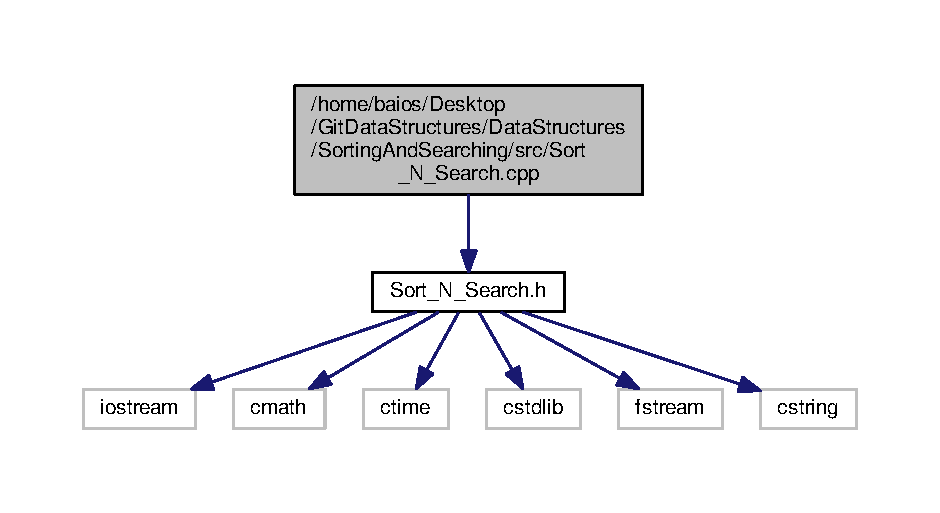
\includegraphics[width=350pt]{_sort___n___search_8cpp__incl}
\end{center}
\end{figure}

%--- End generated contents ---

% Index
\newpage
\phantomsection
\addcontentsline{toc}{chapter}{Index}
\printindex

\end{document}
